\subsection{$d(K^-, n)$ scaling factor}
$d(K^-, n)"X"$ spectrum can be converted from counts to the differential cross section ($\frac{d^2\sigma}{d\Omega dm}$) excepting the acceptance of the the CDS that is depend on the reaction.
The parameters was used for the conversion were summarized in Table\ref{tab:KN_scale}.

First one is luminosity which was consist of number of target, number of irradiated kaon, DAQ live rate, trigger efficeincy.
The number of target was defined from length of fiducial volume ($10cm$) and target density which was evaluated from measured tempature.
The number of irradiated kaon was defined by correcting kaon number counted up by the scaler DAQ by ratio of true kaon in kaon trigger which was described in Sec\ref{sec:beam_line_ana}.
About DAQ live rate and trigger efficiency were discribed in Sec\ref{sec:trigger}.
The luminosity was evaluated run-by-run.
In the table, these items were represented value weighted by data statistics as typical value.

Next is about the CDS which was CDC efficiency discribed in Sec\ref{sec:CDC_eff}.
Accpectances of CDS were estimated and corrected by the Monte Carlo simulation data.
These evaluations were described in individual section for each reactions.

Last one is about the NC which was consists of acceptance and efficiency.
The efficiency of the NC was further decomposed to intrinsic one and overveto by the CVC and the BVC that was described in Sec\ref{sec:NC_eff}.
The acceptance of the NC was estimated from the NC position and the error was evaluated from difference of the first layer and the last layer of the NC.

\input{analysis/KN_scaling_table}


\begin{table}
  \caption{
    Summary table of $d(K^-, p)$ scaling parameters
  }

  \hspace{-2cm}
  \begin{tabular}{cc|cc|cc}
    \multicolumn{2}{c|}{Component}  & value            & error           & value  & error \\
    \hline
    \hline
    Luminosity   ($/\mu b$)    &    & 2478             & 81          &  & \\
    & Target Length (cm)       &  & & 10               &                  \\
    & Target density $[g/cm^3]$&  & & 0.1624           & 0.0014           \\
    & Number of Kaon           &  & & 2.05$\times 10^{10}$ &              \\
    & Survival ratio of $K^-$  &  & & 0.336            & 0.0001           \\
    & DAQ live ratio           &  & & 0.821            & 0.0001           \\
    \multicolumn{2}{c|}{Trigger efficiency}  &  & &                  &    \\
    \hline
    & $K \otimes$CDH1          &  & & 0.9527           & 0.0003 \\
    & Charge                   &  & & 0.9559           & 0.0004 \\
    \hline
    \hline
    Efficiency of the CDC      &    & 0.977            & 0.04    &  & \\
    \hline
    %% \hline
    %% Acceptance of the PC/CVC (msr) & & \multicolumn{4}{|c}{Evaluate by the SIM} \\
    \hline
    Efficeincy of the forward detectors  &    & 0.819            & 0.042   &  & \\
    Efficeincy of the FDC1               &    & 0.987            & 0.005   &  & \\
  \end{tabular}
  \label{table:KP_scaling}
\end{table}


\begin{figure}[htbp]
  \centering
  \includegraphics[width=8cm]{../pic/Run78/KP_ana/solid_ang_144.eps}
  \caption{
    This figure shows the effective rates of solid angle elements in the 1.44–1.45 GeV $\pi^-\Sigma^0$ mass bin,
    as estimated by Monte Carlo simulations.
  }
  \label{fig:PCCVC_SA_elem}
\end{figure}

\begin{figure}[htbp]
  \centering
  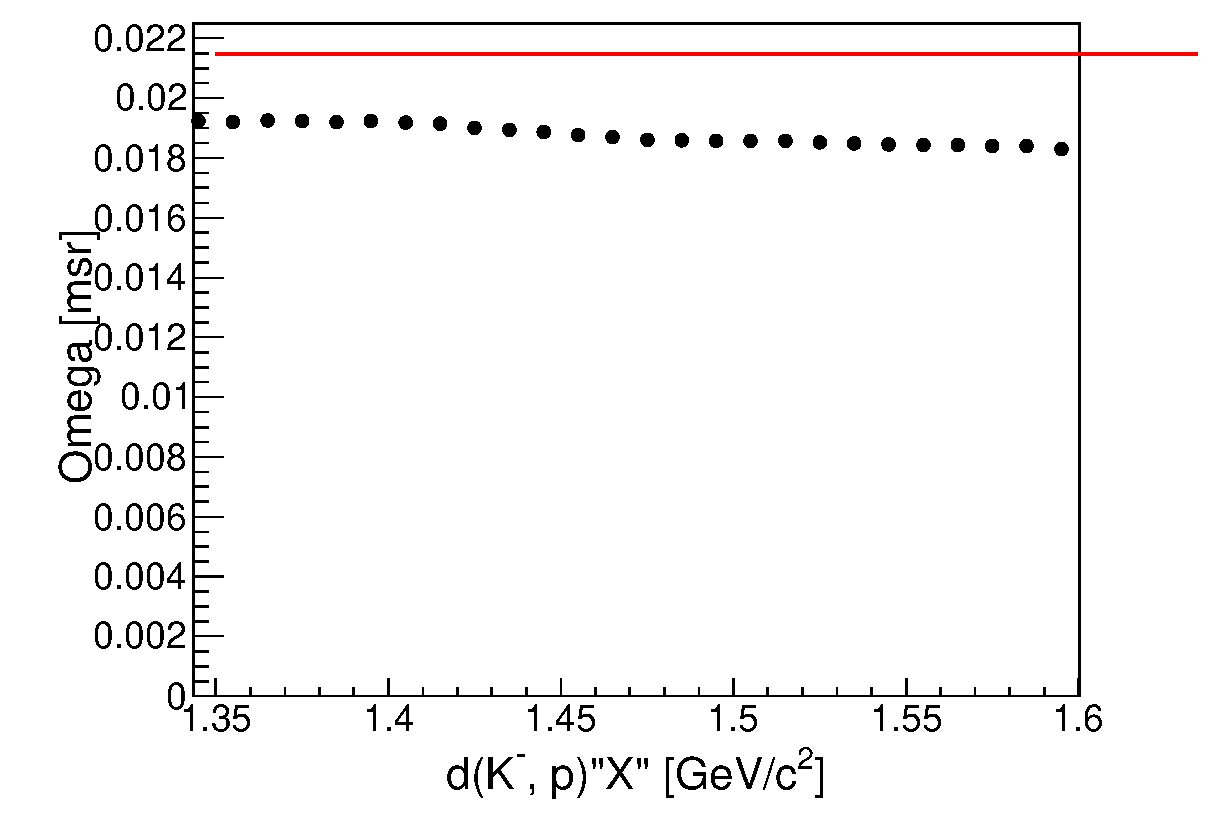
\includegraphics[width=8cm]{../pic/Dron/PCCVC_SA.eps}
  \caption{
    This figure shows the relationship between the mass of the $\pi^-\Sigma^0$ system and
    the solid angles of the forward detectors (FDC1 and PC/CVC) with respect to the outgoing forward proton.
    The red line indicates the solid angle of the NC detector with respect to the forward neutron.
  }
  \label{fig:PCCVC_SA}
\end{figure}


The factors for converting to double-differential cross sections are explained here.
These can be categorized into the following three components:
\begin{enumerate}
\item Luminosity, which is determined by the number of incident beam particles and the number of target nuclei;
\item The solid angle and detection efficiency of the forward-scattered neutrons (or protons) produced in the reaction;
\item The detection efficiency of detectors.
\end{enumerate}

These are summarized in Tables \ref{table:KN_scaling} and \ref{table:KP_scaling} for the forward neutron and forward proton cases, respectively.

Luminosity is a quantity that represents the product of the number of incident beam particles and the number of target particles.
The beam intensity is evaluated by multiplying the beam scaler counts by the DAQ live ratio,
described in Section \ref{sec:DAQ_eff}, which accounts for the fraction of data actually recorded for analysis;
the trigger efficiency, described in Section \ref{sec:trig_eff}, which accounts for whether a trigger signal was actually generated;
and the fraction of $K^-$ beam triggers that passed through the fiducial volume of the target, as described in Section \ref{sec:beam_ana}.
This beam-related quantity is calculated and summed on a run-by-run basis.
Tables \ref{table:KN_scaling} and \ref{table:KP_scaling} show representative values
consisting of the average over all runs and the errors evaluated from the fluctuations.
For the number of target particles, the density of the liquid deuterium target is estimated from the monitored temperatures,
as described in Section \ref{sec:target} The uncertainty is evaluated based on fluctuations during the production run and
is calculated by multiplying the density by the length of the fiducial volume.

% The temperature of the liquid deuterium target is monitored, as described in Section \ref{sec:target},
% and this value is used to evaluate its density.

In the case of forward neutrons, since they travel in straight trajectories,
the solid angle can be defined by the area covered by the NC. When the solid angle is evaluated at the center of the NC
and the variation is assessed by shifting the evaluation point front and back, it is determined to be 21.5 $\pm$ 0.2 [msr]\%.
The detection efficiency of the neutron detector can be divided into two components
the intrinsic detection efficiency of the NC for neutrons and the over-veto effect by the CVC.
The intrinsic neutron detection efficiency is evaluated to be 31.7 $\pm$ 1.6 [\%] using the reaction
$K^- p \rightarrow K^0 n \rightarrow \pi^+ \pi^- n$ with a liquid hydrogen target, as described in Section \ref{sec:NC_eff}.
The over-veto effect in the CVC, which is also considered to be strongly influenced by beam-induced background,
is evaluated to be 8.1 $\pm$ 0.7 [\%] using the production run data, also described in Section \ref{sec:NC_overveto}.

In the case of forward protons, since they are bent by the Usniwaka magnet,
the solid angle coverage depends on the momentum of the forward-scattered proton, i.e., the mass of the $\pi^-\Sigma^0$ system.
To estimate this, we use a dataset similar to the Monte Carlo simulation used for the acceptance correction.
The solid angle for a given $\pi^-\Sigma^0$ mass region is evaluated by dividing the angular space into small solid angle elements.
For each element,
the detection efficiency of the forward detector system (CVC/PC) is evaluated based on whether the proton can actually be detected.
The effective solid angle for each element is then calculated by multiplying the element's solid angle by its detection efficiency,
as shown in Figure \ref{fig:PCCVC_SA_elem}
Finally, the total solid angle is obtained by summing these effective solid angles over all elements, as shown in Figure \ref{fig:PCCVC_SA}.
The solid angle does not change significantly in the region of interest.

In this data set, hadronic reactions and similar processes that could cause secondary interactions are turned off
to avoid double-counting losses already accounted for in the detection efficiency of forward protons evaluated in Section \ref{sec:PC_eff}.
Here, the detection efficiency of protons was estimated to be 81.9 $\pm$ 4.2 [\%] using the $K^- d \rightarrow \pi^- \pi^- p p$ reaction.
Also,
the detection efficiency of FDC1 was evaluated to be 98.7 $\pm$ 0.5 [\%] using the BVC as the trigger detector under the pion beam conditions,
as described in Section \ref{sec:FDC1_eff}.

After applying the CDS acceptance obtained in the previous subsection and the correction factors described here,
we obtain the $d(K^-, n)\pi^{\mp}\Sigma^{\pm}$ and $d(K^-, p)\pi^-\Sigma^0$ cross sections,
as shown in Figures \ref{fig:Charge_CS} and \ref{fig:pimS0_CS}, respectively.

% \begin{frame}{Cross Section of $d(K^-, n)"n K^0"$}
  \begin{figure}
    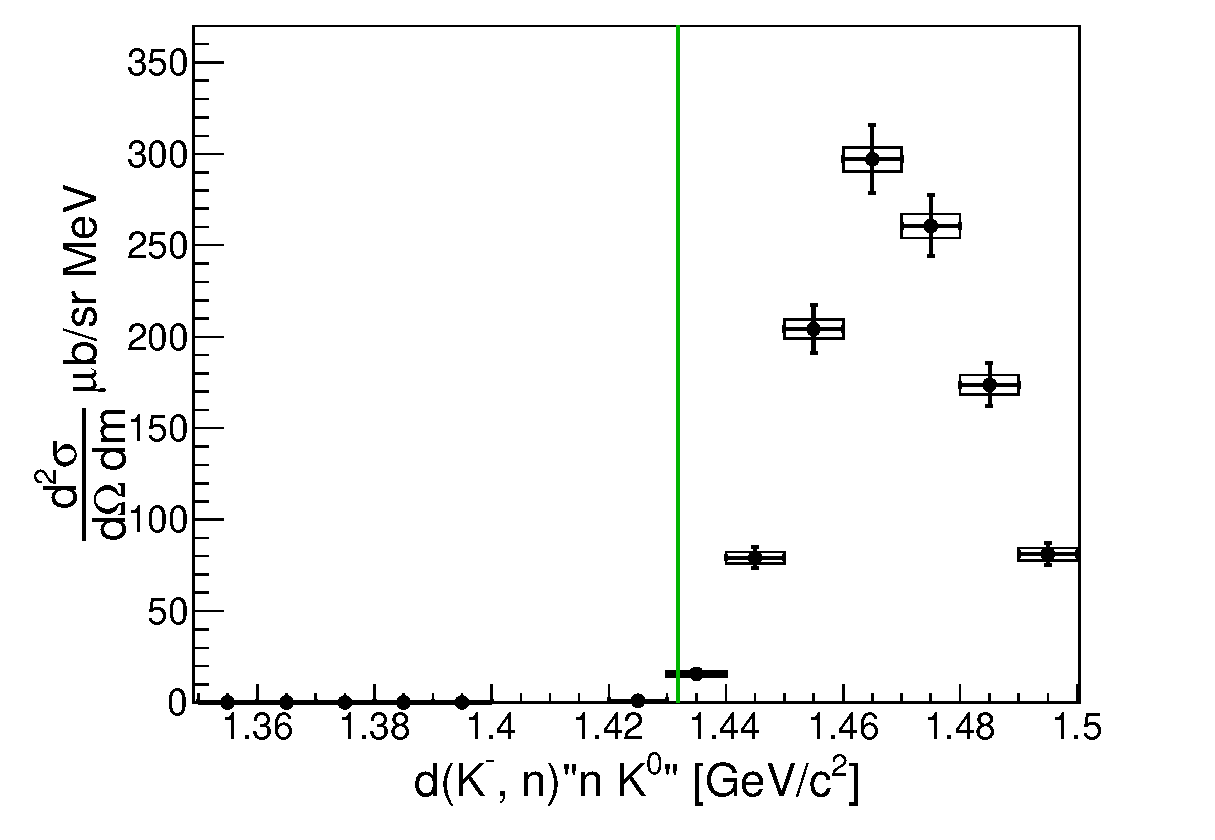
\includegraphics[width=8cm]{../pic/Run78/QE/K0_CS.eps}
  \end{figure}
  \centering
  Box indicates staticial errors.
%%  BG was subtracted.
\end{frame}

\begin{figure}[htbp]
  \centering
  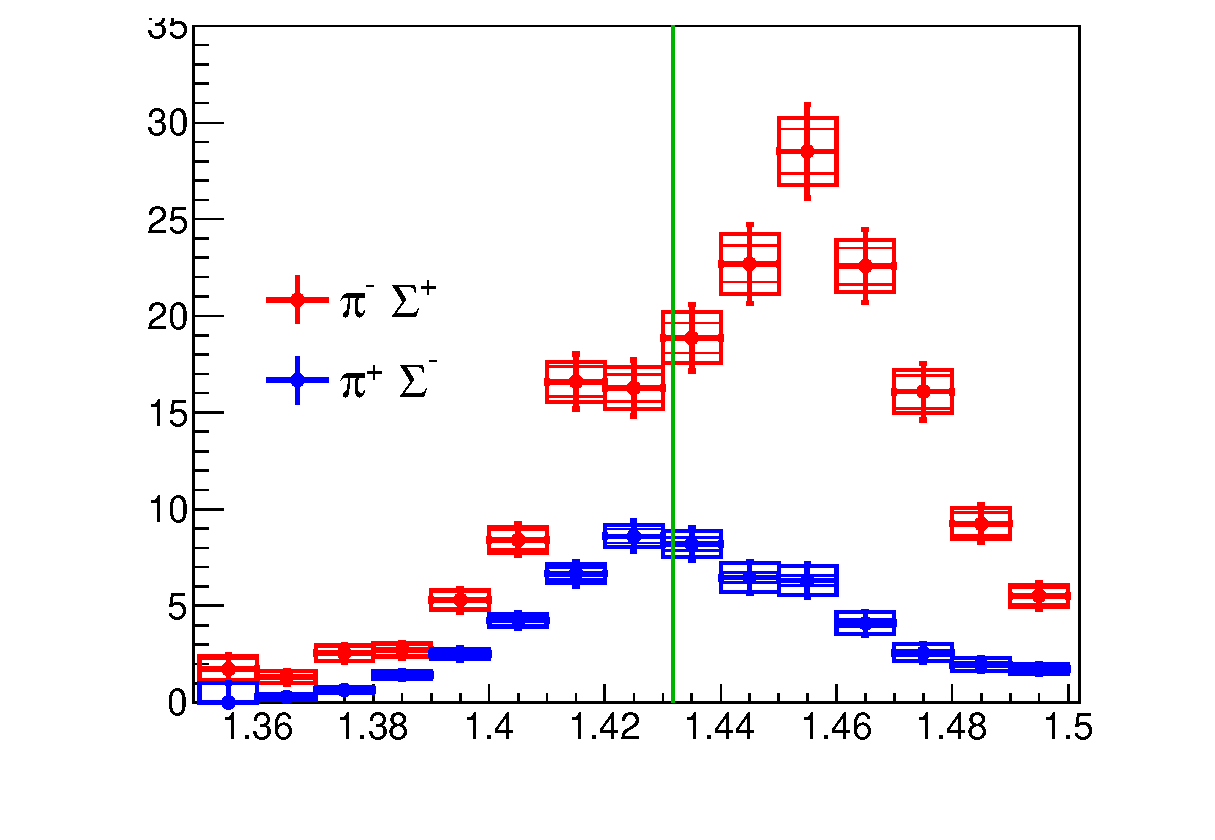
\includegraphics[width=9cm]{../pic/Dron/KN_ana/ChargeCS.eps}
  \caption{
    The red figure and blue figure shows about $d(K^-, n)"\pi^+\Sigma^-"$ and $d(K^-, n)"\pi^-\Sigma^+"$, respectively.
    The inner frame (thin line), outer frame (thick line), and error bars represent the addition of statistical errors, fitting errors, and conversion errors, which were calculated by root-mean-square.
    The green vertical lines indicates $\bar{K}N$ threshold.
  }
  \label{fig:Charge_CS}
\end{figure}

\begin{figure}[htbp]
  \centering
  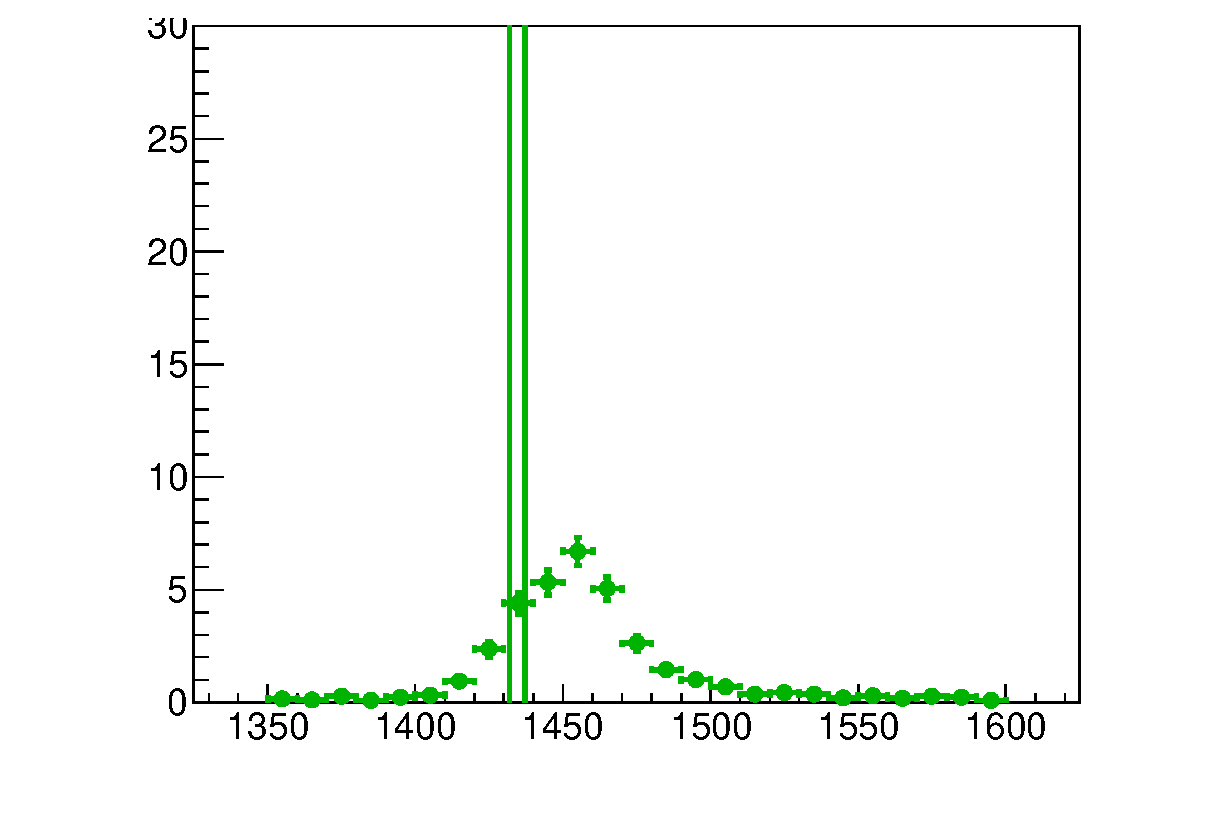
\includegraphics[width=9cm]{../pic/Dron/KP_ana/pimS0_CS.eps}
  \caption{
    This figure shows the cross section of $d(K^-, p)"\pi^- \Sigma^0"$.
    The box represents the statistical error, and the error bar represents the root mean squares of the conversion factor added to it.
    The green vertical lines indicates $\bar{K}N$ threshold.
  }
  \label{fig:pimS0_CS}
\end{figure}










%% The solid angle for a given $\pi^-\Sigma^0$ mass region is evaluated by summing the effective solid angles,
%% each weighted by the detection efficiency of the forward detector system (CVC/PC), over the solid angle bins of the generated protons.

%% In this data set, hadron reactions and other reactions are turned off to prevent double-counting of losses due to reactions included in the detection efficiency of forward protons evaluated in Section 2.3.


%% The obtained spectra are converted to cross sections.
%% For this purpose, the target, beam, and DAQ efficiencies are summarized as luminosity.
%% The target and beam quantities are discussed in Sections.\ref{sec:target} and \ref{sec:Kbeam}, respectively.
%% The DAQ efficiency consists of two parts, one of which is the DAQ live rate and the other is the trigger efficiency, described in Sections.\ref{sec:DAQ_live_rate} and \ref{sec:trigger}.
%% Detector efficiency is also evaluated and corrected for conversion to cross sections.
%% The CDC, NC, and PC efficiencies are described in Sections.\ref{sec:CDC}, \ref{sec:NC}, and \ref{sec:PC}, respectively. 
%% These conversion factors are common for the $\pi \Sigma$ spectra.
%% These factors are summarized in Table.\ref{table:KN_scaling} and Table.\ref{table:KP_scaling} about $d(K^-, n)$ and $d(K^-, p)$, respectively.

%% On the other hand, the acceptances depend on the $\pi \Sigma$ mass spectra.
%% % In the case of $d(K^-, n)"\pi^{\mp} \Sigma^{\pm}"$, the separation ratio of $\pi^- \Sigma^+$ and $\pi^+ \Sigma^-$ is also depend on.
%% We obtain the cross section of $d(K^-, n)"n K^0"$, $d(K-, n)"\pi^-\Sigma^0"$ and $d(K^-, p)"\pi^- \Sigma^0"$ by adapting the these corrections,
%% which are shown in Figure.\ref{fig:nK0_CS}, Figure.\ref{fig:Charge_CS}, and Figure.\ref{fig:pimS0_CS}, respectively.
%% We obtain the cross section of $d(K-, n)"\pi^-\Sigma^0"$ and $d(K^-, p)"\pi^- \Sigma^0"$ by adapting the these corrections,
%% which are shown in Fig.\ref{fig:Charge_CS}, and Fig.\ref{fig:pimS0_CS}, respectively.

% \begin{figure}[htbp]
  \centering
  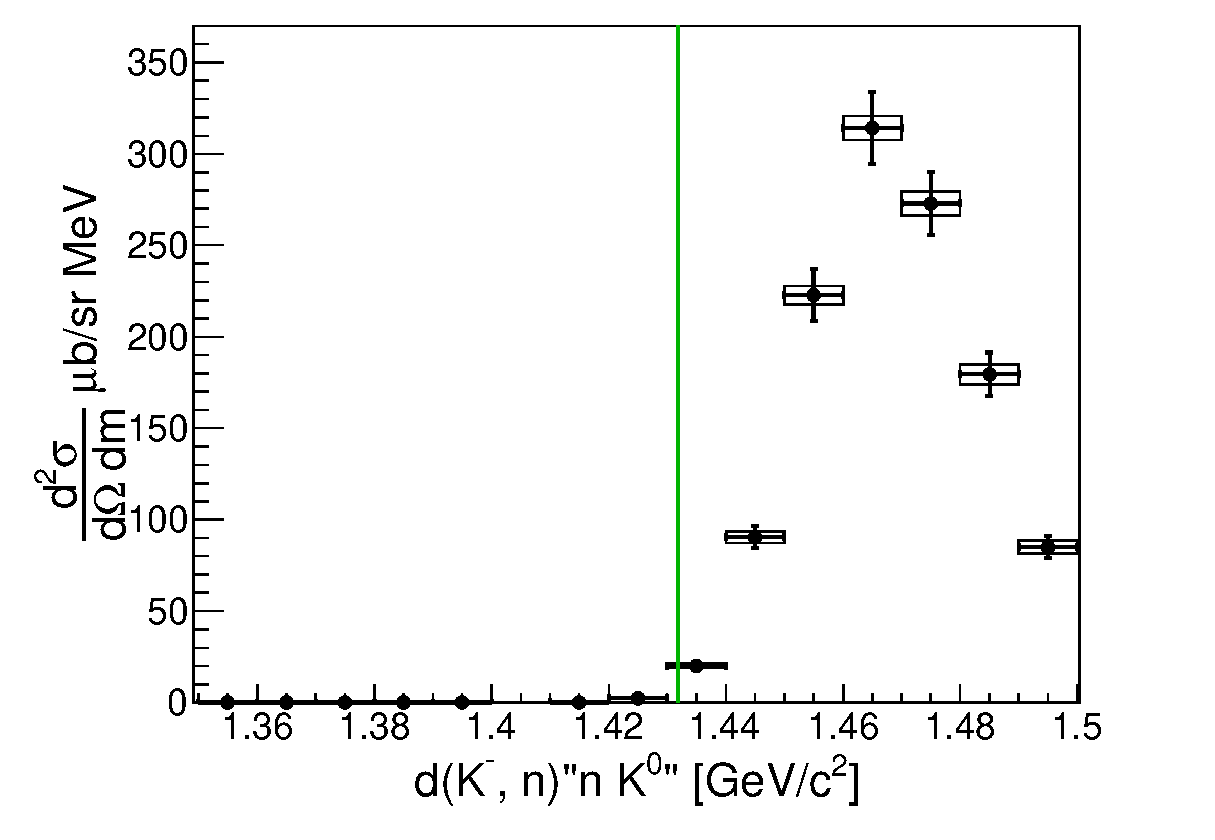
\includegraphics[width=6cm]{../pic/Dron/K0_ana/K0_CS.eps}
  \caption{
    This figure shows the cross section of $d(K^-, n)"n K^0"$.
    The box represents the statistical error, and the error bar represents the root mean squares of the conversion factor added to it.
    The green vertical lines indicates $\bar{K}N$ threshold.
  }
  \label{fig:nK0_CS}
\end{figure}

\begin{figure}[htbp]
  \centering
  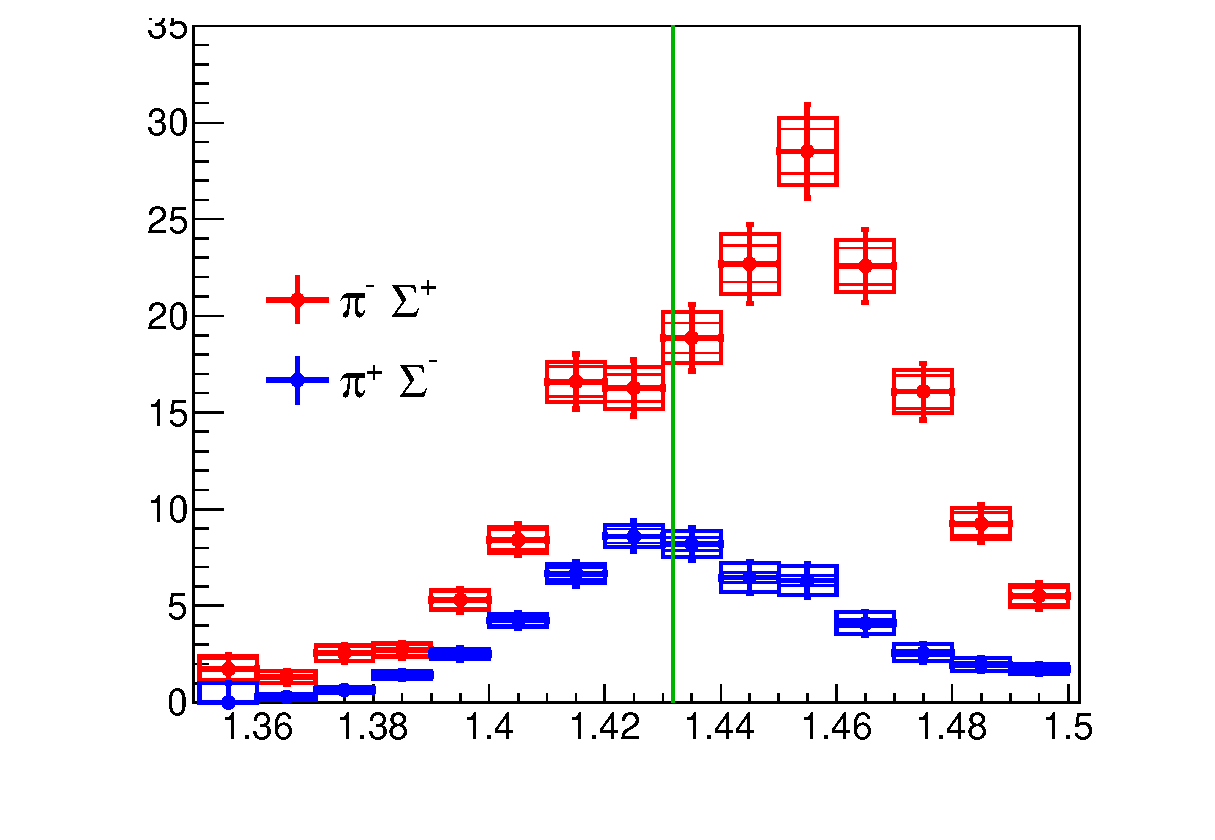
\includegraphics[width=6cm]{../pic/Dron/KN_ana/ChargeCS.eps}
  \caption{
    The red figure and blue figure shows about $d(K^-, n)"\pi^+\Sigma^-"$ and $d(K^-, n)"\pi^-\Sigma^+"$, respectively.
    The inner frame (thin line), outer frame (thick line), and error bars represent the addition of statistical errors, fitting errors, and conversion errors, which were calculated by root-mean-square.
    The green vertical lines indicates $\bar{K}N$ threshold.
  }
  \label{fig:ChargeCS}
\end{figure}

\begin{figure}[htbp]
  \centering
  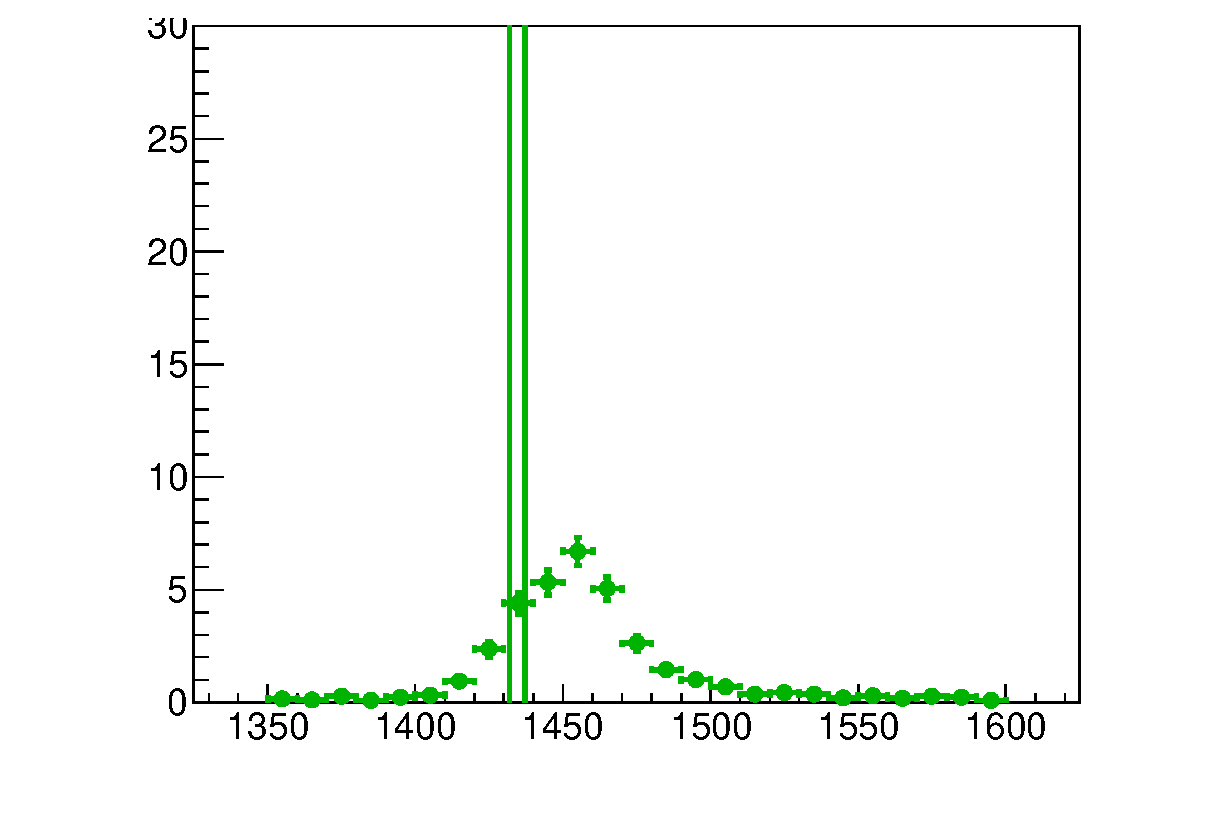
\includegraphics[width=6cm]{../pic/Dron/KP_ana/pimS0_CS.eps}
  \caption{
    This figure shows the cross section of $d(K^-, p)"\pi^- \Sigma^0"$.
    The box represents the statistical error, and the error bar represents the root mean squares of the conversion factor added to it.
    The green vertical lines indicates $\bar{K}N$ threshold.
  }
  \label{fig:pimS0_CS}
\end{figure}


% We discuss the physical mean about obtained spectra.
